% +------------------------------------------------------------------------+
% | Reference manual page: Halfedge.tex
% +------------------------------------------------------------------------+
% | 17.03.1999   Lutz Kettner
% | Package: Polyhedron
% | 
\RCSdef{\RCSHalfedgeRev}{$Revision$}
\RCSdefDate{\RCSHalfedgeDate}{$Date$}
% +------------------------------------------------------------------------+

\ccRefPageBegin

%%RefPage: end of header, begin of main body
% +------------------------------------------------------------------------+


\begin{ccRefClass}[Polyhedron_3<Traits>::]{Halfedge}

\ccDefinition
  
Figure~\ccTexHtml{\ref{figurePolyOptionalMethods} on page 
\pageref{figurePolyOptionalMethods}}{}\begin{ccHtmlOnly}
  <A HREF="#figurePolyOptionalMethods"><IMG 
  SRC="cc_ref_up_arrow.gif" ALT="reference arrow" WIDTH="10" HEIGHT="10"></A>
\end{ccHtmlOnly}
depicts the relationship between a halfedge and its incident
halfedges, vertices, and facets.  A halfedge is an oriented edge
between two vertices. It is always paired with a halfedge pointing in
the opposite direction. The \ccc{opposite()} member function returns
this halfedge of opposite orientation. If a halfedge is incident to a
facet the \ccc{next()} member function points to the successor
halfedge around this facet. For border edges the \ccc{next()} member
function points to the successor halfedge along the hole. For more
than two border edges at a vertex, the next halfedge along a hole is
not uniquely defined, but a consistent assignment of the next halfedge
will be maintained in the data structure. An invariant is that
successive assignments of the form \ccc{h = h->next()} cycle
counterclockwise around the facet (or hole) and traverse all halfedges
incident to this facet (or hole). A similar invariant is that successive
assignments of the form \ccc{h = h->next()->opposite()} cycle
clockwise around the vertex and traverse all halfedges incident to
this vertex. Two circulators are provided for these circular orders.

\begin{ccTexOnly}
    \begin{figure}[bht]
        \begin{center}
          \parbox{\textwidth}{%
              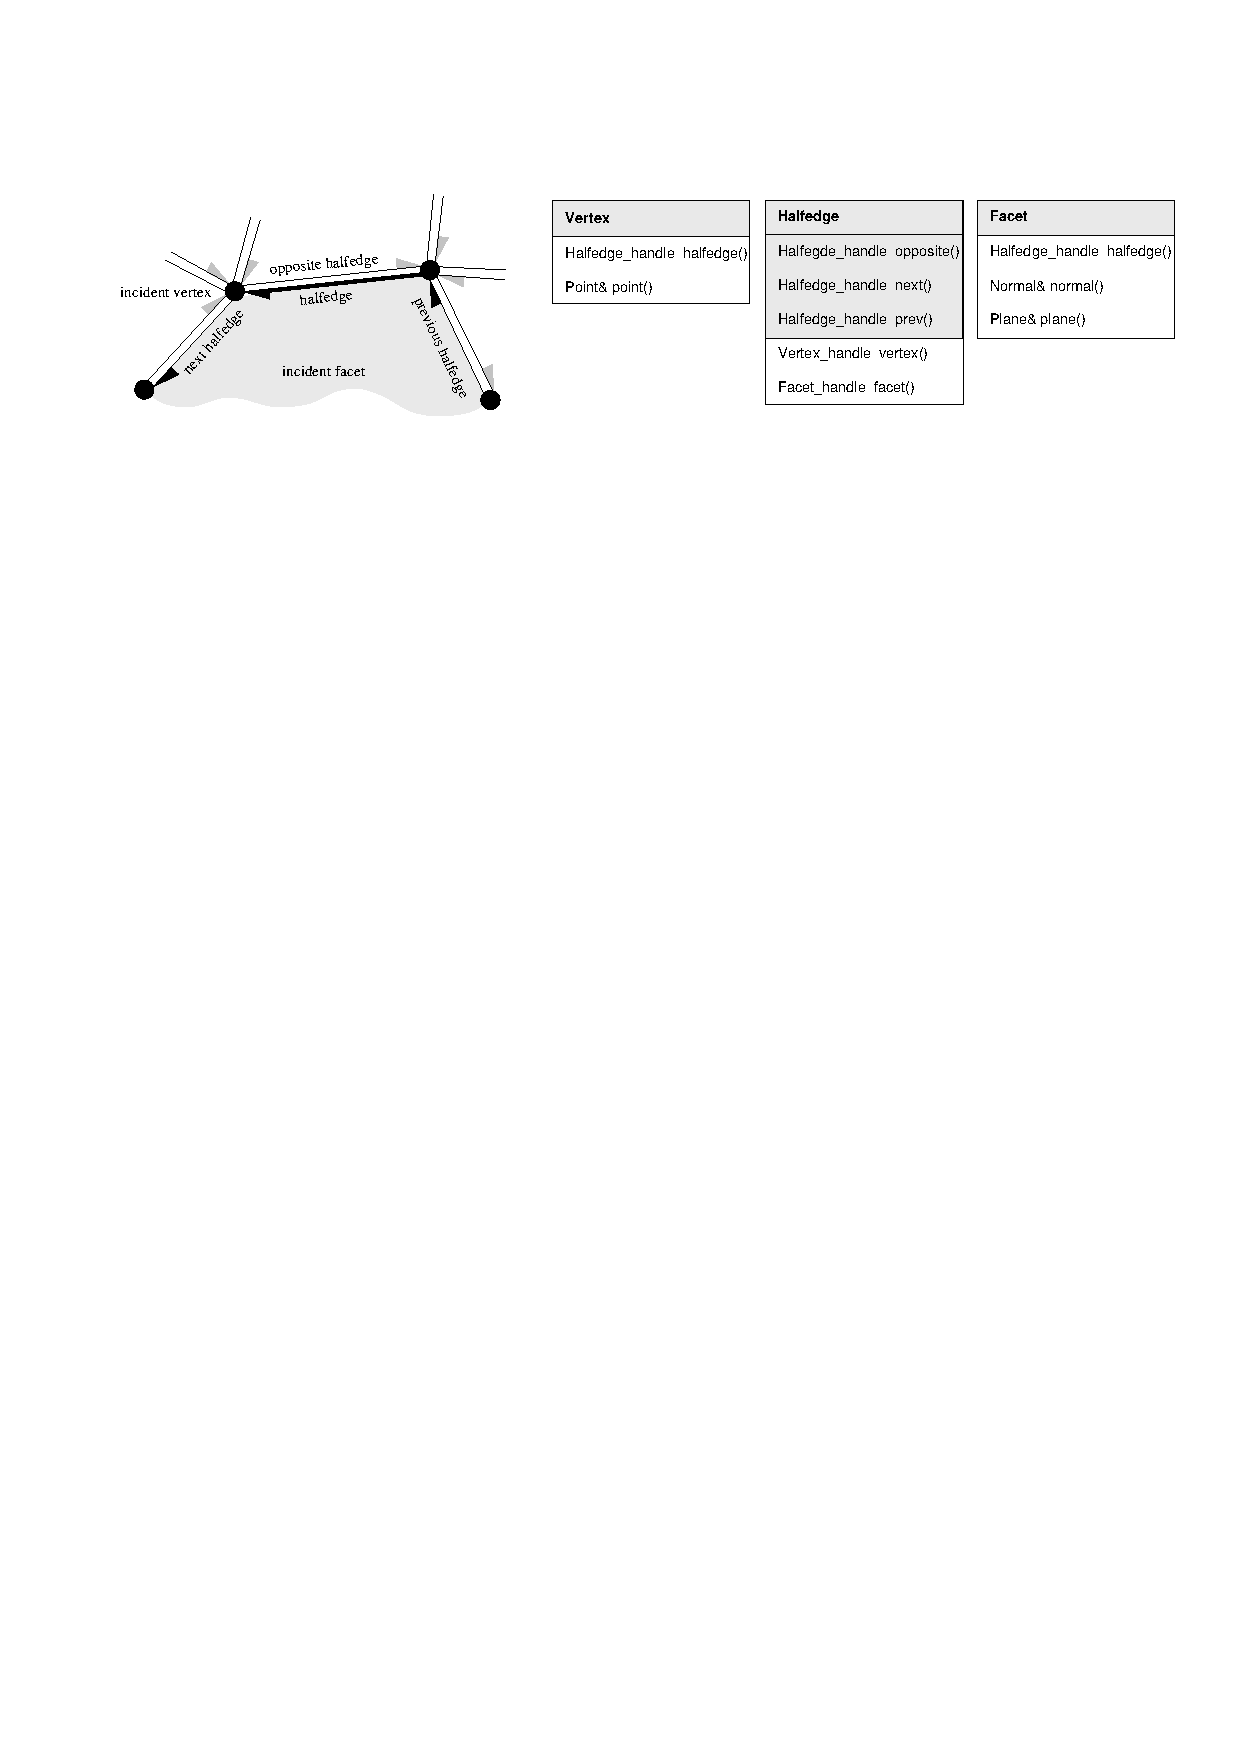
\includegraphics[width=\textwidth]{fig/poly_optional.ips}%
          }
        \end{center}
        \caption{The three classes \protect\ccc{Vertex}, 
          \protect\ccc{Halfedge}, and 
          \protect\ccc{Facet} of the polyhedral surface. Member
          functions with shaded background are mandatory. The others
          are optionally supported.}
        \label{figurePolyOptionalMethods}
    \end{figure}
\end{ccTexOnly}

\begin{ccHtmlOnly}
    <CENTER>
    <A NAME="figurePolyOptionalMethods">
    <A HREF="./poly_optional.gif">
        <img src="./poly_optional_small.gif" 
             alt="Class Diagram"></A><BR>
    <A HREF="./poly_optional.gif">Figure:</A>
    The three classes <I>Vertex</I>, <I>Halfedge</I>, and 
          <I>Facet</I> of the polyhedral surface. Member
          functions with shaded background are mandatory. The others
          are optionally supported.
    </CENTER>
\end{ccHtmlOnly}


The incidences encoded in \ccc{opposite()} and \ccc{next()} are
available for each instantiation of polyhedral surfaces.  The other
incidences are optionally available as indicated with type tags.  The
\ccc{prev()} member function points to the preceding halfedge around
the same facet. It is always available, though it might perform a
search around the facet using the \ccc{next()} member function to find
the previous halfedge if the underlying halfedge data structure does
not provide an efficient \ccc{prev()} member function for halfedges.
Handles to the incident vertex and facet are optionally stored.

The circulators are assignable to the \ccc{Halfedge_handle}. The
circulators are bidirectional if the halfedge provided to the
polyhedron with the \ccc{Items} template argument provides a member
function \ccc{prev()}, otherwise they are of the forward category.


\ccInclude{CGAL/Polyhedron_3.h}

\vspace*{-1mm}
\ccTypes
\ccThree{Halfedge_const_handle}{h.next_on_vertex() const;;}{}
\ccThreeToTwo

\ccNestedType{Vertex}{type of incident vertices.}
\ccGlue
\ccNestedType{Facet}{type of incident facets.}
\vspace*{-3mm}

\ccNestedType{Vertex_handle}{handle to vertex.}
\ccGlue
\ccNestedType{Halfedge_handle}{handle to halfedge.}
\ccGlue
\ccNestedType{Facet_handle}{handle to facet.}
\ccGlue
\ccNestedType{Halfedge_around_vertex_circulator}{circulator of
  halfedges around a vertex.}
\ccGlue
\ccNestedType{Halfedge_around_facet_circulator}{circulator of
  halfedges around a facet.}

\ccNestedType{Vertex_const_handle}{}
\ccGlue
\ccNestedType{Halfedge_const_handle}{}
\ccGlue
\ccNestedType{Facet_const_handle}{}
\ccGlue
\ccNestedType{Halfedge_around_vertex_const_circulator}{}
\ccGlue
\ccNestedType{Halfedge_around_facet_const_circulator}{}

\ccNestedType{Supports_halfedge_prev}{$\equiv$ \ccc{CGAL::Tag_true} or 
  \ccc{CGAL::Tag_false}.}
\ccGlue
\ccNestedType{Supports_halfedge_vertex}{$\equiv$  \ccc{CGAL::Tag_true} or 
  \ccc{CGAL::Tag_false}.}
\ccGlue
\ccNestedType{Supports_halfedge_face}{$\equiv$  \ccc{CGAL::Tag_true} or 
  \ccc{CGAL::Tag_false}.}


\ccCreation
\ccCreationVariable{h}

\ccConstructor{Halfedge();}{default constructor.}

\ccTagFullDeclarations
\ccOperations

\ccMethod{Halfedge_handle opposite();}{}
\ccGlue
\ccMethod{Halfedge_const_handle opposite() const;}{the opposite halfedge.}

\ccMethod{Halfedge_handle next();}{}
\ccGlue
\ccMethod{Halfedge_const_handle next() const;}
    {the next halfedge around the facet.}

\ccMethod{Halfedge_handle prev();}{}
\ccGlue
\ccMethod{Halfedge_const_handle prev() const;}
    {the previous halfedge around the facet.}

\ccMethod{Halfedge_handle next_on_vertex();}{}
\ccGlue
\ccMethod{Halfedge_const_handle next_on_vertex() const;}{
    the next halfedge around the vertex (clockwise). Is equal
    to \ccc{h.next()->opposite()}.}

\ccMethod{Halfedge_handle prev_on_vertex();}{}
\ccGlue
\ccMethod{Halfedge_const_handle prev_on_vertex() const;}{
    the previous halfedge around the vertex (counterclockwise). 
    Is equal to \ccc{h.opposite()->prev()}.}

\ccMethod{bool             is_border() const;}
    {is true if \ccVar\ is a border halfedge.}
\ccGlue
\ccMethod{bool             is_border_edge() const;}
    {is true if \ccVar\ or \ccc{h.opposite()} is a border halfedge.}


%%\ccThree{Halfedge_const_handleh.next_on_vertex() con}{st;;}{}
\ccMethod{Halfedge_around_vertex_circulator       vertex_begin();}{}

\ccMethod{Halfedge_around_vertex_const_circulator vertex_begin() const;}
    {circulator of halfedges around the vertex (clockwise).}

\ccMethod{Halfedge_around_facet_circulator       facet_begin();}{}

\ccMethod{Halfedge_around_facet_const_circulator facet_begin() const;}
    {circulator of halfedges around the facet (counterclockwise).}
%%\ccThree{Halfedge_const_handle}{h.next_on_vertex() const;;}{}

\ccHeading{Operations available if \ccc{Supports_halfedge_vertex} $\equiv$ 
           \ccc{CGAL::Tag_true}}

\ccMethod{Vertex_handle       vertex();}{}
\ccGlue
\ccMethod{Vertex_const_handle vertex() const;}{the incident vertex of \ccVar.}

\ccHeading{Operations available if \ccc{Supports_halfedge_facet} $\equiv$ 
           \ccc{CGAL::Tag_true}}

\ccMethod{Facet_handle       facet();}{}
\ccGlue
\ccMethod{Facet_const_handle facet() const;}
    {the incident facet of \ccVar.  If \ccVar\ is a border halfedge 
      the result is default construction of the handle.}


\ccSeeAlso

\ccRefIdfierPage{CGAL::Polyhedron_3<Traits>::Vertex}\\
\ccRefIdfierPage{CGAL::Polyhedron_3<Traits>::Facet}\\
\ccRefIdfierPage{CGAL::Polyhedron_3<Traits>}

% +-----------------------------------+
\ccImplementation

The member functions \ccc{prev()} and \ccc{prev_on_vertex()} work in
constant time if \ccc{Supports_halfedge_prev} $\equiv$
\ccc{CGAL::Tag_true}. Otherwise both methods search for the previous
halfedge around the incident facet.

\ccTagDefaults
\end{ccRefClass}

% +------------------------------------------------------------------------+
%%RefPage: end of main body, begin of footer
\ccRefPageEnd
% EOF
% +------------------------------------------------------------------------+
